% CREATED BY DAVID FRISK, 2016
\chapter{Methods}
When discussing \textit{accessibility} of a teaching material, in this study, it has been separated into two aspects: \textit{obtainability} and \textit{usability}. A method was developed for collecting usability data, but to accomodate for collecting obtainability data, this method was slightly modified when implementing it.
%
%\section{Obtainability}
%Obtainability describes how easy it is for a teacher to obtain a teaching material, and the data for this aspect of accessibility has mainly be acquired through studying literature. Some data connected to obtainability has also been acquired while performing usability testing, partly because these aspect have proven hard to isolate from each other.
%
%\section{Usability}
The following methodology describes the foundation of the methodology used in this study, as well as a methodology one can use when revising their own shareable teaching material.

\section{The KRUT-methodology}
While deciding on the aim of this study, a new methodology was developed for usability testing. The methodology was named KRUT, from the processes involved; \textbf{K}ick-off meeting, \textbf{R}evising material, \textbf{U}sability \textbf{T}esting. Developing KRUT helped clarify what the study did and did not aim to investigate and how that was expected to play out. As with ASD, KRUT includes a learning loop. The main purpose of KRUT is to use data collected by usability testing a teaching material to revise said material. Usability testing fills two roles; \textbf{identifying \textit{satisfactory} usability} as well as \textbf{identifying \textit{potential gains in} usability}. KRUT also describes the roles of the different actors, based on the current stage of the testing phase. It is designed with a team of two and a single subject group in mind. The KRUT-methodology is described in Figure~\ref{workflow}.

\begin{sidewaysfigure}
\centering
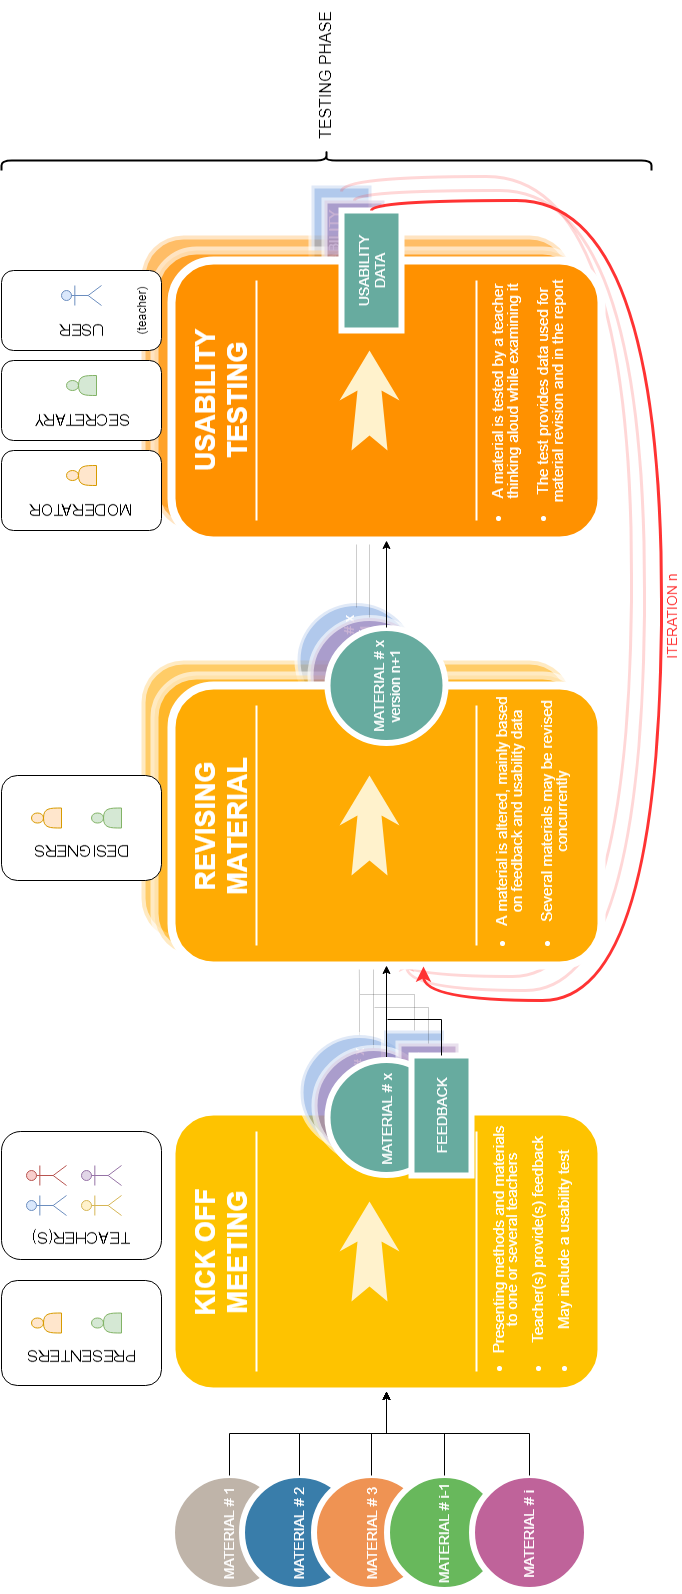
\includegraphics[scale=0.6,angle=-90]{figure/krut.png}
\vspace*{2cm}
\caption{The custom KRUT-methodology, created for usability testing teaching materials}
\label{krut}
\end{sidewaysfigure}

\subsubsection*{Comparing ASD to KRUT} 
There are both similarities and differences when comparing ASD to the KRUT methodology presented in Figure~\ref{asd} and Figure~\ref{krut}. 

The \textbf{Kick Off Meeting} used to introduce one or more teachers to the study, as well as deciding on a teaching material to work on and a date for the first usability test, is comparable to the \textbf{\textit{Project Initiation}} of ASD, being prior to the steps contained inside the \textbf{\textit{Learning Loop}}.

What in the ASD methodology is called \textbf{\textit{Adaptive Cycle Planning}} is the initial step of the \textbf{Revising Material} stage, deciding on how to rework the teaching material based on the data collected from a \textbf{Kick Off Meeting} or previous \textbf{Usability Test}. This is inevitably one of the stages where collected data is summarized and analyzed, even if just as a thought process.

The \textbf{\textit{Concurrent Component Engineering}} part of ASD is practically the same as the \textbf{Revising Material} stage. This is where a coder would revise the code of the program and this is likewise where the product, the teaching material, is being worked on with the intent of improving its usability.

What is called \textbf{\textit{Quality Review}} in ASD is the \textbf{Usability Testing} part of KRUT. This is where the teaching material is tested on a teacher and the data needed to improve the usability of the teaching material is collected. The method used to test usability is based on Steve Krug’s script for usability testing websites. Because a teaching material is quite different from a website, oftentimes focusing on interactivity, the script could not be used without some changes. There is however some important aspects of Steve Krug’s script, e.g. not asking leading questions, that is of great importance to the quality of the data and thereby the quality of future revisions of the teaching material. (Krug, 2009)

The end goal of ASD is called \textbf{\textit{Final QA and Release}}. In the case of KRUT, this step has been reduced. Its original intent is to finalize a product, whereas KRUT defines every revision as an equally valid product, even though the latest revision would theoretically be the most desired.

\subsection{Implementation of KRUT}
Test subjects consisted of individual teachers and teacher students, instead of a team (or teams) of teachers, as would have been desired. Because of this, and to collect more data concerning the obtainability aspect, each usability tests began with a stripped down version of a Kick Off Meeting. This meant that the subject was able to choose from a detailed list what teaching material they wanted to use for their usability test. This list was compiled specifically for this study and consisted of sample teaching materials produced at \todo{mention Kleindagarna earlier or describe more here. /H} Kleindagarna. This was done as a compromise between delimiting the study and offering teaching materials that felt relevant to the teachers. Even though KRUT was designed to be implemented by a team of two, there were no severe difficulties in executing KRUT when the team at times was forced to only one member.

When revising material, the decisions of what to revise when is determined by a combination of data from usability tests and by studying literature. \todo{The later part of this paragraph brings up something we don't do. /H}There may have been instances where a teacher’s assumptions of how the next revision will look have been unmet. These cases need to be analyzed and mentioned in the final report, as they may lead to interesting discussions. If for example a revision is made following a certain pedagogic template, and the resulting material makes the test subject less inclined to use it on a lesson, new conclusions can possibly be drawn about accessibility of designing teaching materials.


\subsection{Test subject anonymity} \label{subjectanonymity}
There are several ways of presenting the personal details of test subjects in scientific studies. In this study some personal details have been disclosed and some have been held anonymous. What is disclosed and examples of what is held anonymous are listed below.

\subsubsection*{Disclosed information}
    \begin{itemize} %Disclosed information
    \item Age – rounded to nearest 5 years.
    \item Current status – if the test subject is currently working as a teacher and if so on what stage of education, or if they are e.g. studying to become a teacher.
    \item Years in teaching – nearest year if under 10 years, can otherwise be rounded to nearest 5 years. No regard to the age of students taught. No regard to full-time or part-time employment.
    \item Subjects – what school subjects is the test subject certified to teach or studying to teach?
\end{itemize}

\subsubsection*{Anonymous information}
\begin{itemize} %Anonymous information
    \item Sex/Gender – the risk of a reader finding false correlations from the data is assumed to be greater if the test subject’s sex and/or gender is disclosed.
    \item Name – the name of the test subjects will not be disclosed, and because the sex/gender will not either, the label of the test subjects will also be as gender free as possible.
    \item Name of school – with this information, it would be too easy to identify the test subject.
    \item Place of school – all subjects studied will live and work in close proximity to Gothenburg, Sweden, as it has been decided to delimit the tests to personal meetings.
\end{itemize}
